\documentclass[conference]{IEEEtran}
\usepackage{booktabs} % For formal tables
\usepackage{caption}
%\usepackage{subfig}
\usepackage{subcaption}
\usepackage{placeins}
\usepackage{xcolor}
\usepackage{float}
\usepackage{url}
\usepackage{epstopdf}
\usepackage{graphics,graphicx}
%\usepackage{cite}%
%\usepackage{epsfig}
\usepackage{array}
\usepackage{pifont}
\usepackage{multirow}
%\usepackage{fixltx2e}
\usepackage{amssymb}
\usepackage{amsmath}
%\usepackage{footnote}
%\usepackage[ruled]{algorithm2e}
%\usepackage{amssymb}
%\usepackage{algorithmic}
\usepackage{algorithm, algpseudocode}

\usepackage{paralist, tabularx}

\usepackage{color}
\newcommand{\red}[1]{\textcolor{red}{#1}}
\newcommand{\todo}[1]{\textcolor{red}{TODO: #1}}
\newcommand{\new}[1]{\textcolor{blue}{#1}}
\newcommand{\doubt}[1]{\textcolor{red}{DOUBT: #1}}


\begin{document}

\title{Fairness for Whom? Understanding the Reader's Perception of Fairness in Text Summarization}
%\title{Please do not edit now!!!- Abhisek}

% author names and affiliations
% use a multiple column layout for up to three different
% affiliations

\author{\IEEEauthorblockN{Anurag Shandilya, Abhisek Dash}
\IEEEauthorblockA{
Indian Institute of Technology Kharagpur, India
}
\if 0
\and
\IEEEauthorblockN{Abhisek Dash}
\IEEEauthorblockA{
Computer Science and Engineering \\ 
Indian Institute of Technology Kharagpur, India%\\
%dash.abhi93@iitkgp.ac.in
}
\fi 
\and
\IEEEauthorblockN{Abhijnan Chakraborty}
\IEEEauthorblockA{Max Planck Institute for Software Systems, Germany%\\
%achakrab@mpi-sws.org
}
\and
\IEEEauthorblockN{Kripabandhu Ghosh}
\IEEEauthorblockA{
Indian Institute of Science Education and Research Kolkata, India%\\
%kripaghosh@iiserkol.ac.in
}

\and
\IEEEauthorblockN{Saptarshi Ghosh}
\IEEEauthorblockA{
Indian Institute of Technology Kharagpur, India%\\
%saptarshi@cse.iitkgp.ac.in
}
}

\if 0 
\IEEEoverridecommandlockouts
\IEEEpubid{\makebox[\columnwidth]{978-1-7281-6251-5/20/\$31.00~\copyright2020 IEEE \hfill} \hspace{\columnsep}\makebox[\columnwidth]{ }}
\fi 
% make the title area
\maketitle

%\IEEEpubidadjcol


% As a general rule, do not put math, special symbols or citations
% in the abstract
\if 0 
\begin{abstract}
There has been an exponential increase in the information shared and posted over social networks. As the user-generated textual information grows rapidly, there has been a parallel uptick in the use of summarization algorithms for providing an overview of the extensive content. Traditional metrics for measurement of the quality of summarization algorithms rely on matching machine generated summaries to human-generated ones (ROUGE scores for example). However, it has been shown that when the textual data comes from various socially salient groups; for eg. men or women, caucasians or African-Americans, the summarization algorithms represent the social groups very differently compared to their distribution in the original data. Abhishek et al ~\cite{dash2019summarizing} have also proposed various fairness-preserving summarization algorithms to mitigate these adverse impacts. However, all of these studies have considered normative notions of fairness and that too from the side of the producers of the content to be summarised. We propose a descriptive framework for looking into the problem of fairness in summarization from the side of the consumers of the summarised information.
\end{abstract}
\fi 

\begin{abstract}
With the surge in user-generated textual information, there has been a recent increase in the use of summarization algorithms for providing an overview of the extensive content. 
Traditional metrics for evaluation of these algorithms (e.g. ROUGE scores) rely on matching algorithmic summaries to human-generated ones. However, it has been shown that when the textual contents are heterogeneous, e.g., when they come from different socially salient groups, most existing summarization algorithms represent the social groups very differently compared to their distribution in the original data. To mitigate such adverse impacts, some fairness-preserving summarization algorithms have also been proposed. 
All of these studies have considered normative notions of fairness from the perspective of writers of the contents, neglecting the readers' perceptions of the underlying fairness notions. To bridge this gap, in this work, we study the interplay between the fairness notions and how readers perceive them in textual summaries. 
Through our experiments, we show that reader's perception of fairness is often context-sensitive. Moreover, standard ROUGE evaluation metrics are unable to quantify the perceived (un)fairness of the summaries. 
To this end, we propose a human-in-the-loop metric and an automated graph-based methodology to quantify the perceived bias in textual summaries. We demonstrate their utility by quantifying the (un)fairness of several summaries of heterogeneous socio-political microblog datasets.\footnote{\textcolor{red}{This work has been accepted at International Workshop on Fair and Interpretable Learning Algorithms 2020 (FILA 2020), which was held in conjunction with IEEE BigData 2020. Please cite the version appearing in the proceedings.}}
\end{abstract}

% no keywords

% For peer review papers, you can put extra information on the cover
% page as needed:
% \ifCLASSOPTIONpeerreview
% \begin{center} \bfseries EDICS Category: 3-BBND \end{center}
% \fi
%
% For peerreview papers, this IEEEtran command inserts a page break and
% creates the second title. It will be ignored for other modes.
\IEEEpeerreviewmaketitle

\section{Introduction}\label{sec:intro}
% Multi-armed bandit (MAB) is a classic sequential decision making problem \citep{auer2002finite}, where a learning agent chooses among competing actions sequentially to maximize its accumulative reward over time. 
% %Despite its simplicity, MAB exemplifies the exploration-and-exploitation dilemma that also exists in more complicated problems. 
% An important extension of MAB, named linear contextual bandit \citep{li2010contextual}, incorporates contextual information in the problem setting, by assuming a linear mapping between the context and expected reward. It has gained popularity in various applications, such as recommender systems \citep{li2010contextual}, display advertisement \citep{li2010exploitation} and clinical trials \citep{durand2018contextual}.
% Most existing linear bandit solutions are designed under a centralized learning setting, i.e., data is readily available at a central server. However, with the increasing public concerns of privacy, especially the bandit algorithms usually directly learn from user data,
% %more and more people are reluctant to provide their own data and strict regulations on data usage like GDPR have also went into effect \cite{voigt2017eu}, which makes 
% there is a growing demand to keep data decentralized and push the learning of bandit models to the client side. 
% % This idea is also made much more feasible due to the growing computational power of edge devices nowadays. 

% Federated learning has recently emerged as a promising setting for decentralized machine learning.
% % , and its effectiveness was first validated at a large scale by training a global model across all mobile devices via the Google Keyboard Android application \cite{konevcny2016federated}. 
% %The term ``federated learning" was first introduced by \citet{mcmahan2017communication} with an emphasis on efficiently training deep models over mobile device applications. As significant amount of later works have applied federated learning to other applications, there may be variations in its meaning for different research communities. 
% Since its debut in \citet{mcmahan2017communication}, there have been variations in its definition for different applications \citep{yang2019federated}.
% In this paper, we follow the general definition by \citet{kairouz2019advances}: multiple clients collaborate in solving a machine learning problem under the coordination of a central server, while keeping each client's raw data local. 
% So far, most existing works in federated learning study offline supervised learning problems \citep{konevcny2016federated,zhao2018federated}, where labeled training instances already sit on the client side. How to perform bandit learning under the federated learning setting remains underexplored.
As a popular online learning problem, linear contextual bandit has been used for a variety of applications, including recommender systems \citep{li2010contextual}, display advertisement \citep{li2010exploitation} and clinical trials \citep{durand2018contextual}. While most existing solutions are designed under a centralized setting (i.e., data is readily available at a central server), in response to the increasing application scale and public concerns of privacy, there is a growing demand to keep data decentralized and push the learning of bandit models to the client side.
% As a classic sequential decision making problem, linear contextual bandit has been widely used for a variety of real-world applications, including recommender systems \citep{li2010contextual}, display advertisement \citep{li2010exploitation} and clinical trials \citep{durand2018contextual}. 
% Most existing solutions are designed under a centralized learning setting, i.e., data is readily available at a central server. However, with the increasing public concerns of privacy, especially the bandit algorithms usually directly learn from user data,
% there is a growing demand to keep data decentralized and push the learning of bandit models to the client side. 
Federated learning has recently emerged as a promising setting for decentralized machine learning \citep{konevcny2016federated}.
% , and its effectiveness was first validated at a large scale by training a global model across all mobile devices via the Google Keyboard Android application \cite{konevcny2016federated}. 
%The term ``federated learning" was first introduced by \citet{mcmahan2017communication} with an emphasis on efficiently training deep models over mobile device applications. As significant amount of later works have applied federated learning to other applications, there may be variations in its meaning for different research communities. 
Since its debut in \citeyear{mcmahan2017communication}, there have been many variations for different applications \citep{yang2019federated}. However, most existing works study offline supervised learning problems \citep{li2019convergence,zhao2018federated}, which only concerns optimization convergence over a fixed dataset. How to perform federated bandit learning remains under-explored, and is the main focus of this paper. 

Analogous to its offline counterpart, the goal of federated bandit learning is to minimize the cumulative regret incurred by $N$ clients during their online interactions with the environment over time horizon $T$,
% $N$ clients in a learning system need to collaborate to minimize the overall cumulative regret over a finite time horizon $T$, 
while keeping each client's raw data local. Take recommender systems as an example, where the clients correspond to the edge devices that directly interact with user by making recommendations and receiving feedbacks. Unlike centralized setting where observations from all clients are immediately transmitted to the server to learn a single model, in federated bandit learning, each client makes recommendations based on its local model, with occasional communication for collaborative model estimation.

% In this paper, we follow the general definition by \citet{kairouz2019advances}: multiple clients collaborate in solving a machine learning problem under the coordination of a central server, while keeping each client's raw data local. 


%Though having potential for wide range of applications, online learning problems like linear bandit in federated learning setting, a.k.a. federated linear bandits \cite{dubey2020differentially}, have not attracted enough attention and still remain an open problem. 

% Therefore, it is a natural idea to study contextual linear bandit in a federated learning paradigm, which is also referred to as federated linear bandits \cite{dubey2020differentially}. In a federated learning paradigm, multiple clients collaborate in solving a machine learning problem, under the coordination of a central server, and each client's raw data is stored locally and not transferred to the server. 
% when linear bandit algorithms are applied to the federated learning paradigm, because these algorithms assume a traditional centralized machine learning system where all the data are collected together and all the computation happens in one machine or data center. 
Several new challenges arise in this problem setting. 
The first is the conflict between the need of timely data/model aggregation for \emph{regret minimization} and the need of \emph{communication efficiency}, since communication is the main bottleneck for many distributed application scenarios, e.g., communication in a network of mobile devices can be slower than local computation by several orders of magnitude \citep{huang2013depth}. A well-designed communication strategy becomes vital to strike the balance. 
In addition, 
% constraints from real-world applications should also be taken into consideration when designing the communication strategy. For example, 
the clients often have various response time and even occasional unavailability in reality, due to the differences in their computational and communication capacities.
% the clients may differ in their computational and communication capacities. This will lead to various response time and even occasional unavailability. 
This hampers global synchronization employed in existing federated bandit solutions \citep{wang2019distributed,dubey2020differentially}, which requires the server to first send a synchronization signal to all clients, wait and collect their returned local updates, and finally send the aggregated update back to every client.
Second, it is very restrictive to only assume homogeneous clients, i.e., they solve the same learning problem. 
% As bandit algorithms are mostly deployed to interact with individual users, studying heterogeneous clients with personalized learning problems has a greater potential.
Studying \emph{heterogeneous clients} with distinct learning problems has a greater potential in practice.
This is referred to as ``\emph{non-IIDness}" of data in the context of federated learning, e.g., the difference in $\mathcal{P}_{i}(\bx,y)=\mathcal{P}_{i}(\bx) \mathcal{P}_{i}(y|\bx)$ is caused by each client $i\in[N]$ serving a particular user or group of users, a particular geographic region, or a particular time period. Apparently, it is also unreasonable to assume every client has equal amount of new observations, which however is assumed in existing works. 

%To be more concrete, due to the time-varying arm set $\cA_{t}$ and the dependence on history data for arm selection in linear bandit, context vector $X$ is non-IID in nature and is not the main concern. 
% It is not a major concern since the performance metric, i.e. regret $r_{t}$, is defined against the best arm in $\cA_{t}$. 

% For example, internet connection and the different computation power of devices.
% \textcolor{red}{reasons we need async algo}

% This naturally leads to the question: how to balance between regret minimization and communication efficiency in the federated linear bandit problem.
To address the first challenge, we propose an asynchronous event-triggered communication framework for federated linear bandit. 
%Our event-triggering mechanism offers a flexible way to balance between the regret-minimization and communication-efficiency dilemma. 
Communication with a client happens only when the last communicated update to the client becomes irrelevant to the latest one; and we prove only by then effective regret reduction can be expected in this client because of the communication. 
Under this asynchronous communication, each client sends local update to and receives aggregated update from the server independently from other clients, with no need for global synchronization. This improves our method's robustness against possible delays and temporary unavailability of clients. It also brings in reduced communication cost when the clients have distinct availability of new observations, because global synchronization requires every client in the learning system to send its local update despite the fact that some clients can have very few new observations since last synchronization.
% make the proposed method more robust and practical against the infrastructure constraints, because the aggregated update sent to each client is asynchronous and  
% This makes our method more robust against possible delays in the communication, and we prove that the client enjoys the same benefit in regret reduction as long as it receives the update before its next interaction with the environment.

To address the second challenge, we design algorithms for federated linear bandit with both ``\emph{IIDness}" and ``\emph{non-IIDness}" based on the proposed communication framework. We consider two different assumptions on the reward functions. First, all the clients share a common reward function i.e., a single model is learned for all clients. Second, each client has a distinct reward function with mutual dependence captured by globally shared components in the unknown parameter, which resembles 
%so one model per client is learned during the interaction with the environment, which in essence is similar to the problem considered in
federated multi-task learning \citep{smith2017federated}.
We rigorously prove the upper bounds of accumulative regret and communication cost for the proposed algorithms in these two settings, and conduct extensive empirical evaluations to demonstrate the effectiveness of our proposed framework.
% especially its flexibility in balancing the trade-off between regret and communication cost.
%%%%%%%%%%%%%%%%%%%%%%%%%%%%%%%%%%%%%%%%%%%%%%%%%%
\section{Related Works}
\label{main:sec:related}
%%%%%%%%%%%%%%%%%%%%%%%%%%%%%%%%%%%%%%%%%%%%%%%%%%
\gls{cnp}~\citep{garnelo2018conditional} is the first \gls{npf} model which consists of simple \gls{mlp} layers as its encoder and decoder. \gls{np}~\citep{garnelo2018neural} also uses \gls{mlp} layers as its encoder and decoder but introduces a global latent variable to model a functional uncertainty.
\gls{canp}~\citep{kim2018attentive} and \gls{anp}~\citep{kim2018attentive} are the models which apply attention modules as their encoder block in order to well summarize context information relevant to target points. 
\citet{louizos2019functional} proposed \glspl{np} model which employs local latent variables instead of a global latent variable by applying a graph neural network.
By applying convolution layers as their encoder, \citet{gordon2020convolutional} and \citet{foong2020meta} introduced a translation equivariant \glspl{cnp} and \glspl{np} model, respectively. 
In addition to these works, \gls{bnp}~\citep{lee2020bootstrapping} suggests modeling functional uncertainty with the bootstrap~\citep{efron1992bootstrap} method instead of using a single global latent variable. 
% \gls{neubnp}~\citep{lee2022neural} also used a recent bootstrap method called Neural Bootstrapper~\citep{shin2021neural} to model functional uncertainty.


\section{Datasets} 
\label{sec:datasets}
\noindent We reuse the following two datasets from our prior work~\cite{dash2019summarizing}.

\vspace{2mm}
\noindent \textbf{(1) US-Election dataset:} This dataset, originally provided by Darwish et al.\cite{darwish2017trump}, contains English tweets
posted during the 2016 US Presidential election. Each tweet is annotated as supporting or attacking
one of the presidential candidates (Donald Trump and Hillary Clinton) or neutral or attacking both.
For simplicity, we grouped the tweets into three classes: 
(i)~Pro-Republican: tweets which support
Trump and / or attack Clinton, 
(ii)~Pro-Democratic: tweets which support Clinton and / or attack Trump, and 
(iii)~Neutral: tweets which are neutral or attack both candidates. 

%After removing duplicates, we have $2,120$ tweets, out of which $1,309$ (61.74\%) are Pro-Republican, $658$ (31.04\%) tweets are Pro-Democratic, and remaining $153$ (7.22\%) are Neutral tweets.

\vspace{2mm}
\noindent \textbf{(2) MeToo dataset:} We collected a set of tweets related to the MeToo movement in October 2018.
%We initially collected $10,000$ English tweets containing the hashtag MeToo using the Twitter Search API. 
Specifically, we collected English tweets containing the hashtag `\#MeToo' using the Twitter Search API. 
%After removing duplicates, we were left with $3,982$ distinct tweets. 
We asked three human annotators to examine the name and bio of the Twitter accounts who posted the tweets.
The annotators observed three classes of tweets based on who posted the tweets -- (i)~tweets posted by male users, 
(ii)~tweets posted by female users, and
(iii)~tweets posted by organizations (mainly news media agencies). 
Also, there were many tweets for which the annotators could not understand the
type/gender of the user posting the tweet. For purpose of this study, we decided to focus only on
those tweets for which all the annotators were certain that they were written by male users or female users. 
%In total, we had $488$ such tweets, out of which $213$ are written by men and $275$ are written by women.

\vspace{2mm}
\noindent From each of these two datasets, we selected a set of $50$ tweets, having an equal representation of the different demographic groups. In other words, we selected $50$ tweets from the USElection dataset, containing $17$ pro-Democratic tweets, $17$ pro-Republican tweets, and $16$ neutral tweets.
Similarly, we selected $50$ tweets from the MeToo dataset, containing $25$ tweets posted by male users and $25$ tweets posted by female users. 
While selecting these two sets of $50$ tweets, we ensured choosing distinct tweets  (for which we removed near-duplicates) that were well-formed and informative.
All experiments in this paper are conducted over these two sets of $50$ tweets each.


In the rest of this paper, we conduct a number of surveys and experiments on the aforementioned datasets in pursuit of answers to the RQs mentioned in the introduction. 

\if 0
\section{Research Questions} \label{sec:rq}
\noindent
Our primary goal in this work is to investigate the following Research Questions (RQs):

\vspace{2mm}
\noindent \textbf{RQ1:} Is the consumers' perception of fairness/bias in summaries context-dependent? If yes, does it align with the traditional definitions of fairness with respect to demographic groups of the producers? If not, then what forms the basis of consumers' perception of fairness/bias?

\vspace{2mm}
\noindent \textbf{RQ2:} Do traditional metrics for summary quality such as ROUGE scores capture consumers' perception of fairness/bias of summaries?

\vspace{2mm}
\noindent \textbf{RQ3:} Can a metric based on `representation of opinions' better capture consumers' perception of fairness/bias in summaries?\\

\noindent
To answer these research questions, we conduct several surveys involving multiple participants over the USElection and MeToo datasets. The surveys are described in the following sections.
\fi 

\section{Understanding Consumers' Perception of Fairness in Summaries}
\label{sec:consumer-perception}
\noindent
In this section, we investigate the  \textbf{RQ$1$} stated in the introduction-- whether readers' perception of (un)fairness in summaries is context dependent. %Section~\ref{sec: intro}. 
To this end, we first generate summaries having different levels of biases, and then conduct a survey to understand how consumers (human annotators) perceive the bias/fairness of these summaries. 


\subsection{Generating differently biased summaries}

%We perform a survey on summarization of crowdsourced text on a polarizing topic (US politics). We consider a set of English microblogs (tweets posted on Twitter) related to the 2016 US Presidential elections. The tweets contain a variety of opinions of their authors on the two presidential candidates Donald Trump and Hillary Clinton – some of the tweets support Trump, while others attack Trump; similarly, some tweets support Clinton while others attack her. Details of this dataset are given in Section 2.4 (the USelection dataset). For simplicity, we consider the tweets to be of three opinion classes – (i) Pro-Republican: tweets which support Trump and / or attack Clinton, (ii) Pro-Democratic: tweets which support Clinton and / or attack Trump, and (iii) Neutral: tweets which are neutral or attack both candidates.
\noindent
We consider a set of $50$ tweets from the US elections dataset ($17$ pro-Democratic tweets, $17$ pro-Republican tweets and $16$ neutral tweets), which are not repetitive in nature. We apply the FairSumm algorithm~\cite{dash2019summarizing} on this set of tweets to generate summaries of length $15$ tweets, having a wide variety of bias (from completely biased towards pro-Republican ideology to completely biased towards pro-Democratic ideology). 
To this end, we fix a certain number of neutral tweets, and then vary the number of pro-Republican and pro-Democratic tweets to create variously biased summaries.
Specifically, we create two batches of summaries, one batch with 3 neutral tweets each, and the other batch with 5 neutral tweets each. 

\vspace{2mm}
The first batch of summaries with 3 neutral tweets each, which we term as {\bf FairSumm-US-Batch1}, contains the following summaries (each of length $15$ tweets):
\begin{enumerate}
\item 00 pro-Rep tweets, 12 pro-Dem tweets, 03 neutral tweets -- actually very unfair summary
\item 02 pro-Rep tweets, 10 pro-Dem tweets, 03 neutral tweets -- actually very unfair summary
\item 04 pro-Rep tweets, 08 pro-Dem tweets, 03 neutral tweets
\item 06 pro-Rep tweets, 06 pro-Dem tweets, 03 neutral tweets -- actually very fair summary
\item 08 pro-Rep tweets, 04 pro-Dem tweets, 03 neutral tweets
\item 10 pro-Rep tweets, 02 pro-Dem tweets, 03 neutral tweets -- actually very unfair summary
\item 12 pro-Rep tweets, 00 pro-Dem tweets, 03 neutral tweets -- actually very unfair summary
\end{enumerate}

\vspace{2mm}
The second batch of summaries with 5 neutral tweets each, which we term as {\bf FairSumm-US-Batch2}, contains the following summaries (each of length $15$ tweets):
\begin{enumerate}
\item 00 pro-Rep tweets, 10 pro-Dem tweets, 05 neutral tweets -- actually very unfair summary
\item 02 pro-Rep tweets, 08 pro-Dem tweets, 05 neutral tweets -- actually very unfair summary
\item 04 pro-Rep tweets, 06 pro-Dem tweets, 05 neutral tweets -- actually very fair summary
\item 06 pro-Rep tweets, 04 pro-Dem tweets, 05 neutral tweets -- actually very fair summary
\item 08 pro-Rep tweets, 02 pro-Dem tweets, 05 neutral tweets -- actually very unfair summary
\item 10 pro-Rep tweets, 00 pro-Dem tweets, 05 neutral tweets -- actually very unfair summary
\end{enumerate}

\vspace{2mm}
Similarly we consider a set of $50$ tweets from the MeToo dataset containing $25$ tweets posted by male users and $25$ tweets posted by female users (as stated in Section~\ref{sec:datasets}).
We then apply FairSumm to generate the following summaries of length $15$ tweets each, having a wide variation of bias (from completely biased towards tweets posted by male users to completely biased towards tweets posted by female users).
We call this batch of summaries {\bf FairSumm-MeToo}, which contains the following summaries (each of length $15$ tweets):
\begin{enumerate}
\item 00 Male tweets, 15 Female tweets -- actually very unfair summary
\item 02 Male tweets, 13 Female tweets -- actually very unfair summary
\item 04 Male tweets, 11 Female tweets
\item 06 Male tweets, 09 Female tweets
\item 08 Male tweets, 07 Female tweets -- actually very fair summary
\item 10 Male tweets, 05 Female tweets
\item 12 Male tweets, 03 Female tweets -- actually very unfair summary
\item 14 Male tweets, 01 Female tweets -- actually very unfair summary
\end{enumerate}

\noindent It can be noted that, for all these summaries generated using the FairSumm algorithm, the actual biases are known in terms of the number of tweets included in a summary from the different perspectives. 
We will next check how the bias/fairness of these summaries is viewed by consumers (human annotators).


\begin{table*}
\center
\begin{tabular}{|p{0.95\textwidth}|}
\hline  
Hillary has derogatory titles for anyone not voting for her.\textbackslash
Unlike Hillary, Trump is facing rape charges.\textbackslash Nothing  will deter Trump and he will not stop fighting for you.\textbackslash
Bill Clinton has admitted that Obamacare is bad and Hillary is pissed about it.\textbackslash
Donald Trump claims credit for terrorist acts, just like terrorists.\textbackslash
Hillary is  only one that can make college affordable.\textbackslash
Trump says he has come on top in the Presidential debate.\textbackslash
17 out of 20 people feel that Hillary is winning.\textbackslash
Trump claims that sources that report negatively about his campaign are not to be trusted.\textbackslash
We know the net worth of Hillary, cause she has disclosed her assets.\textbackslash
Hillary thinks she has a solid strategy to defeat ISIS while Trump has none.\textbackslash
Some Trump supporters want him to win so that they can abuse women they want.\textbackslash
Iraq is getting ready for a battle to reclaim Mosul. \\

\hline \hline
Hillary shames everyone and thinks anyone not voting for her is stupid.\textbackslash 
Trump thinks Hillary  is crooked.\textbackslash
 Trump refuses to accept that the current POTUS was born in America \textbackslash
Obamacare is bad and Hillary is not happy with what Bill Clinton said about it.\textbackslash
Hillary doesn’t have the drive to make America great again.\textbackslash
People who are cancelling subscriptions to Dallas and Arizona newspapers are smart.\textbackslash
For people who don’t wanna vote, they need to be told that only Hillary can get rid of their huge college debt.\textbackslash
Trump thinks Hilary has been fighting ISIS without success for years and now it’s time for a change.\textbackslash
Trump thinks Hillary has told lies throughout her life and has sold America’s interests.\textbackslash
The way Hillary is handling the e-mail case, she is unfit for the post of President.\textbackslash
Hillary is a proponent of more love and kindness in America.\textbackslash
Hillary has a solid strategy to defeat ISIS unlike Trump.\textbackslash
Some guys want Trump to win so that they can oppress women.\textbackslash
We should be thankful to every nation that helped bring Paris agreement into action.\textbackslash
Shooting of unarmed Black men is unacceptable.\textbackslash
Every women in this country deserves to be free from harm and fear.\textbackslash
Charlotte should release police video of the Keith Lamont Scott shooting without delay. \\
 
\hline 
\end{tabular}
\caption{\textbf{Set of distinct opinions (separated by \textbackslash) identified by two of the annotators, from the set of tweets related to US Elections.}}
\vspace{-5mm}
\label{tab:opinions}
\end{table*}


\subsection{Understanding consumers' perception of (un)fairness}
\noindent
We start with a group of six annotators (3 males and 3 females) who have substantial knowledge of US politics and the MeToo phenomenon, and are in the age group of 18--30 years. 
We used a questionnaire to ascertain their knowledge of US politics and the MeToo movement. Also the annotators are familiar with use of social media platforms including Twitter, and none of the annotators is an author of this paper.

The annotators were first asked to go over the two sets of $50$ tweets each (one on USElection, and the other on MeToo) and to note down every distinct {\it opinion} expressed in the tweets.
%They were given a short write up on the process of summarization and an introduction to the concept of ideas/opinion as represented by tweet(s). 
An {\it opinion} is defined as a unique idea/information being conveyed by a tweet, hitherto not covered by any other/previous tweet.
Note that the annotators were only shown the text of the tweets; they were {\it not} told anything about the gender / political ideology of the users who authored the tweets. 
%Subsequently, they were asked to go through the shortened version of the US election dataset. Thereafter, they were asked to identify and jot down the ideas as they perceive as being conveyed by the text.
There was no limit to how many opinions they may identify, however each opinion was required to be confined to a maximum of two sentences. 
Table~\ref{tab:opinions} tabulates the opinions identified by two of the six annotators, from the set of $50$ tweets related to the US Elections. 


Thereafter, the annotators are shown the summaries from the FairSumm-US-Batch1, FairSumm-US-Batch2 and FairSumm-MeToo batches in random order. 
They were asked to judge the fairness of each summary, and label each summary with one of the following labels:
\begin{enumerate}
    \item Very Fair Representation
    \item Somewhat Fair Representation
    \item Somewhat Unfair Representation
    \item Very Unfair Representation
\end{enumerate}
Along with labeling each summary, they were also asked to provide a reasoning for their judgement. In other words, they were asked to indicate the factor(s) based on which they were judging a summary to be fair/unfair:
\begin{enumerate}
    \item Fair/unfair representation of political/gender groups
    \item Fair/Unfair representation of political/contextual opinions
    \item Fair/Unfair representation of both: political/gender groups and political/contextual opinions
    \item Any other reason (requires a subjective response)
\end{enumerate}


%Finally, the above survey was repeated for the shortened version(50 tweet length) of the MeToo Dataset as well.

%In the section we proceed to answer \textbf{RQ$1$} from the surveys. 
Now we examine how the consumer’s perception of fairness varies across different contexts/scenarios. 
To this end, we plot the fraction of annotators who have annotated a summary as either `very fair representation' of the input text, or as `very unfair representation' of the input text. 
These two fractions are termed as `very fair approval fraction' and `very unfair approval fraction' respectively. 

Figure~\ref{Fig: AnnotationDatasets} depicts the result for the USElection dataset (sub-figures (a) and (b) for FairSumm-US-Batch1 and FairSumm-US-Batch1 summaries respectively) and for the MeToo dataset (sub-figure (c) for the FairSumm-MeToo summaries). 
Recall that a batch is a group of summaries having the same number of neutral tweets, but varying number of tweets from other perspectives. 

From the results, it is evident that for the US-Election dataset, the fraction of annotators who said that a summary was `very fair' and the fraction of annotators who said that a summary was `very unfair' correlates well with the actual fairness in the FairSumm summaries. For instance, both summaries having much larger number of pro-Republican tweets and summaries having much larger number of pro-Democratic tweets were labeled as `very unfair' by most annotators. Whereas, the summaries having relatively similar numbers of pro-Republican and pro-Democratic tweets were labeled as `very fair' by most annotators.
Thus, for the USElection dataset, the consumers' perception of fairness in the summaries aligns very well with traditional notions of fairness in representing political groups among the producers (those who authored the tweets).

However, for the MeToo dataset (see Figure~\ref{Fig: AnnotationDatasets}(c)), this is not the case. There is no correlation between group-wise representation of tweets posted by male and female users and the  consumers’ perception of fairness of the summaries. 

\begin{figure*}[t]
	\centering
	\begin{subfigure}{0.65\columnwidth}
		\centering
		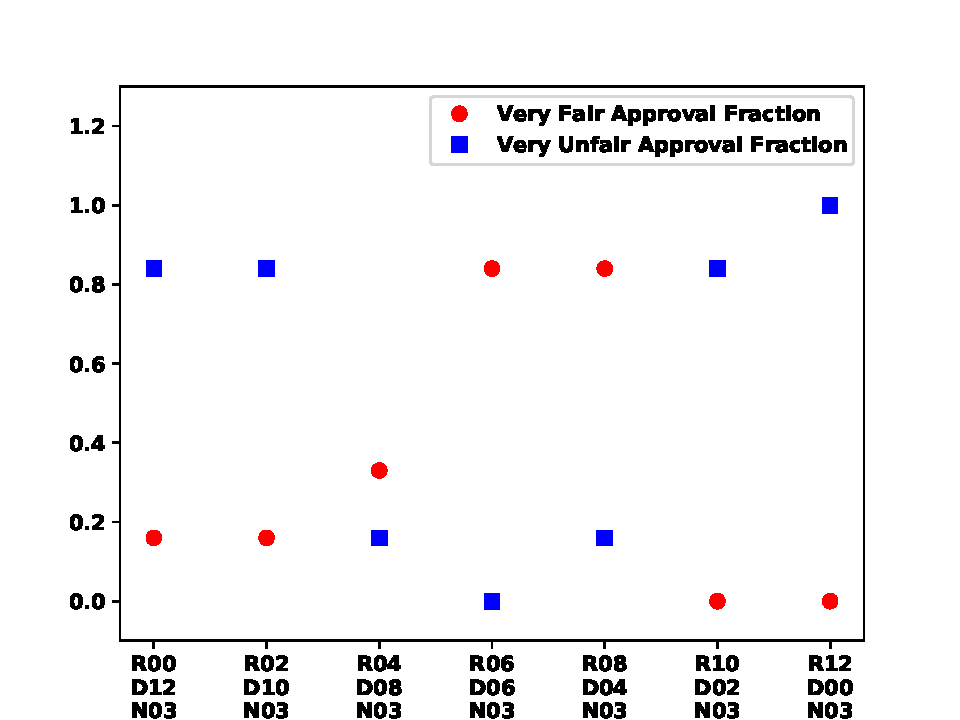
\includegraphics[width=\textwidth, height=3cm]{figures/Sheet1.pdf}
		\vspace*{-3.5mm}
		\caption{\bf FairSumm-US-Batch1 summaries}
		\label{Fig: AnnotationUSEBatch1}
	\end{subfigure}%
	\hfill
	~\begin{subfigure}{0.65\columnwidth}
		\centering
		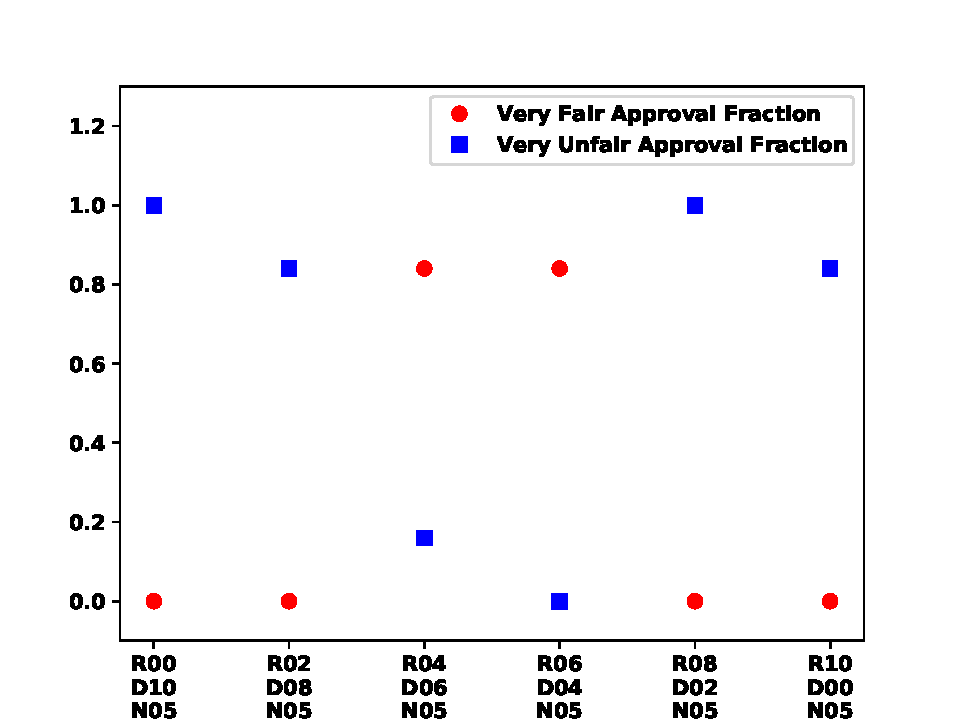
\includegraphics[width=\textwidth, height=3cm]{figures/Sheet5.pdf}
		\vspace*{-3.5mm}
		\caption{\bf FairSumm-US-Batch2 summaries}
		\label{Fig: AnnotationUSEBatch2}
	\end{subfigure}
	\hfill
	~\begin{subfigure}{0.65\columnwidth}
		\centering
		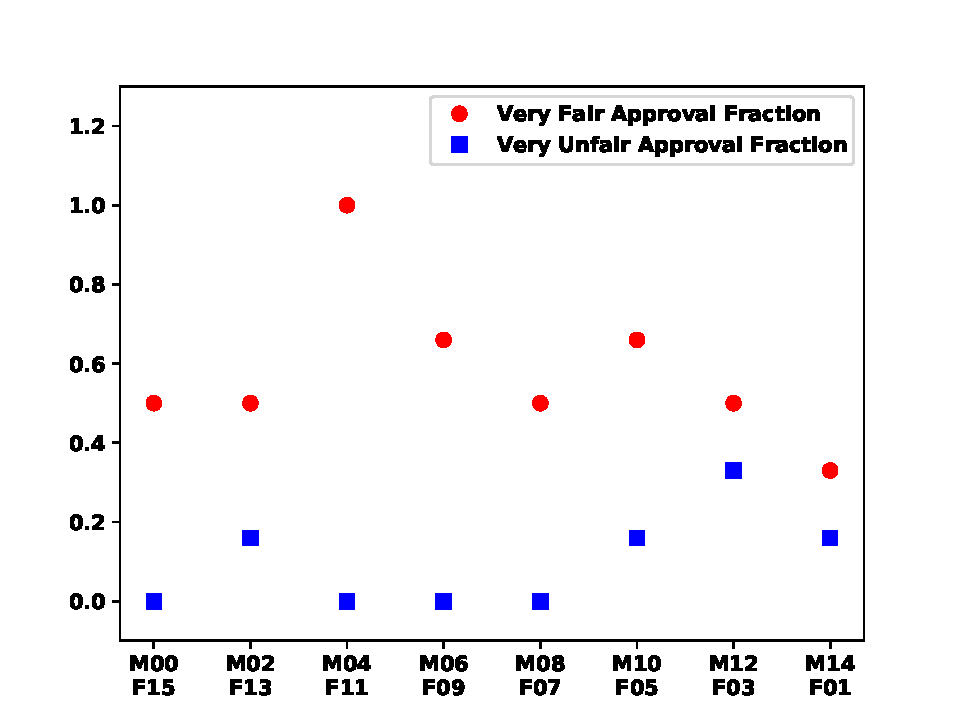
\includegraphics[width=\textwidth, height=3cm]{figures/Sheet9.pdf}
		\vspace*{-3.5mm}
		\caption{\bf FairSumm-MeToo summaries}
		\label{Fig: AnnotationMeToo}
	\end{subfigure}
	
	\caption{{\bf The fraction of consumers (annotators) who labeled various summaries as `Very Fair Representation' (marked by the red circles) and `Very Unfair Representation' (marked by the blue squares) for USElection dataset with (a)~3 neutral tweets, (b)~5 neutral tweets and (c)~for the MeToo dataset. For the USElection dataset, the majority of consumers' perception of (un)fairness agrees with the actual (un)fairness of the summaries. However, the agreement is much lower for the MeToo dataset.}} 
	\label{Fig: AnnotationDatasets}
	
\end{figure*}

This difference for the two datasets leads us to explore more closely why consumers think of a summary as being fair/unfair.


\begin{figure*}[t]
	\centering
	\begin{subfigure}{0.65\columnwidth}
		\centering
		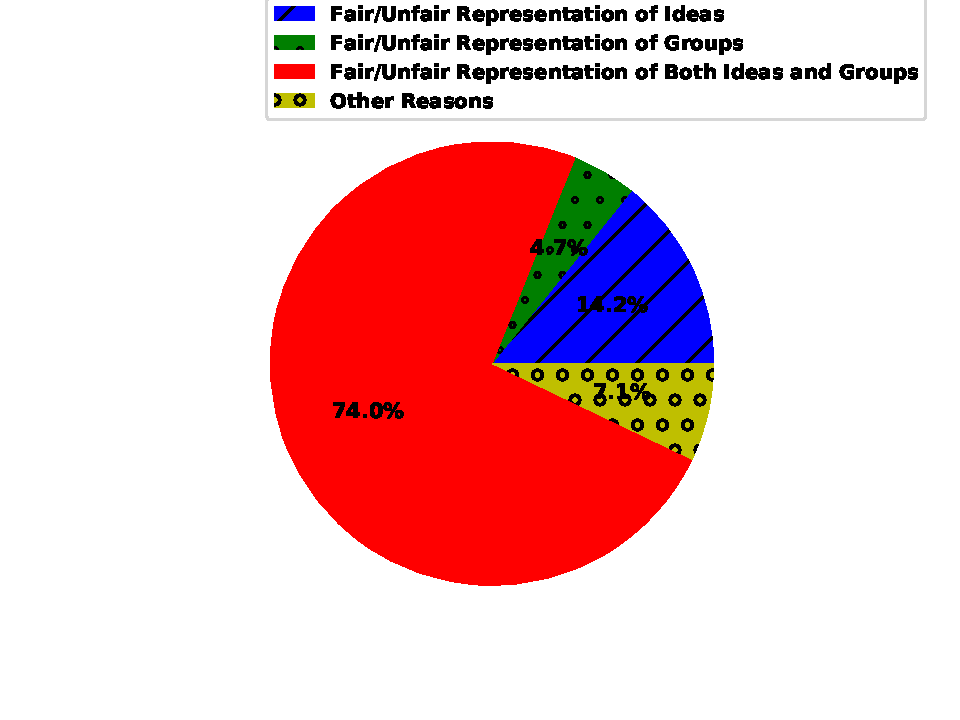
\includegraphics[width=\textwidth, height=4cm]{figures/Sheet15.pdf}
		\vspace{-10mm}
		\caption{\bf FairSumm-US-Batch1 summaries}
		\label{Fig: ReasonUSEBatch1}
	\end{subfigure}%
	\hfill
	~\begin{subfigure}{0.65\columnwidth}
		\centering
		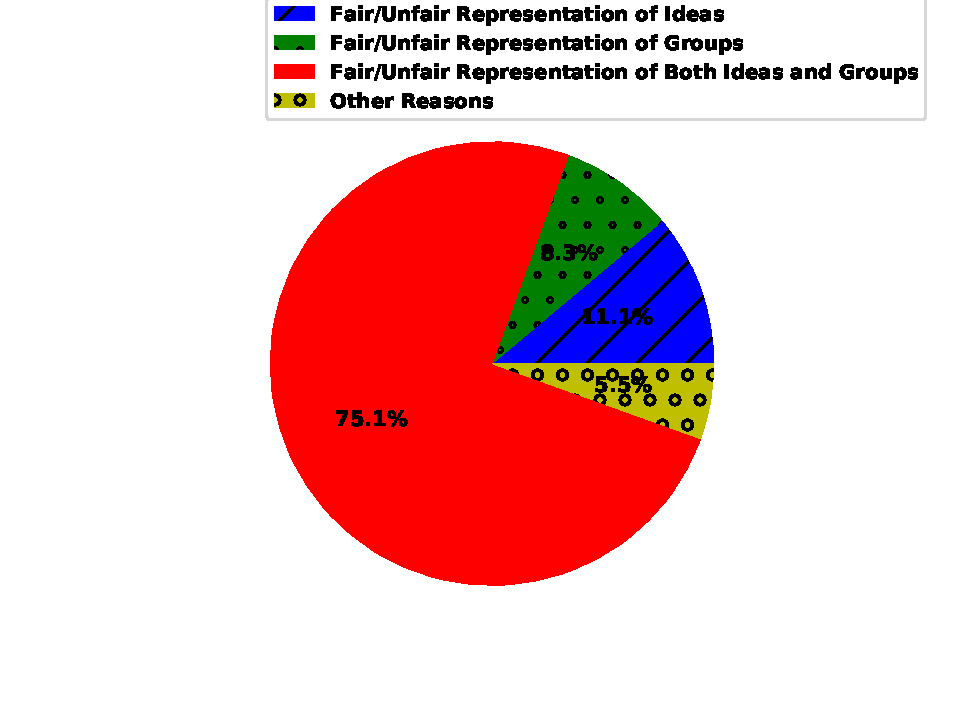
\includegraphics[width=\textwidth, height=4cm]{figures/Sheet14.pdf}
		\vspace{-10mm}
		\caption{\bf FairSumm-US-Batch2 summaries}
		\label{Fig: ReasonUSEBatch2}
	\end{subfigure}
	\hfill
	~\begin{subfigure}{0.65\columnwidth}
		\centering
		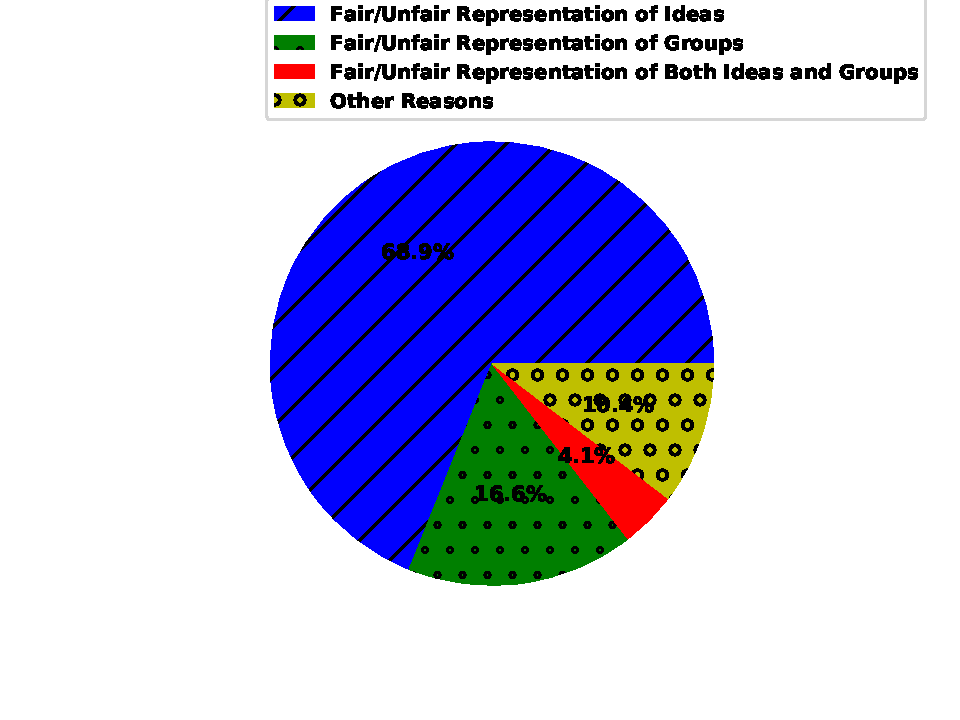
\includegraphics[width=\textwidth, height=4cm]{figures/Sheet13.pdf}
		\vspace{-10mm}
		\caption{\bf FairSumm-MeToo summaries}
		\label{Fig: ReasonMeToo}
	\end{subfigure}
	
	\caption{{\bf The relative proportions of the various reasons given by annotators for judging a summary as fair/unfair for USElection dataset with (a)~3 neutral tweets, (b)~5 neutral tweets and (c)~for the MeToo dataset. We observe that for the USElection dataset, most consumers labeled a summary to be (un)fair based on the (un)fair representation of both political opinions and groups. Whereas, the consumers gave priority to (un)fair representation of opinions in the MeToo dataset.}} 
	\label{Fig: ReasonDataset}
    \vspace{-5mm}
\end{figure*}

\subsection{Why do consumers think of a summary as being (un)fair?}

\noindent
As stated earlier in this section, we also asked the annotators to indicate {\it why} they labeled a certain summary as fair/unfair -- whether they considered the political/gender groups of the users who posted the tweets (which were not specifically told to them), or the political/contextual opinions (which were identified by the annotators themselves), or both, or some other factor. 
We now look at the distribution of the reasons as stated by the annotators. 



Figure~\ref{Fig: ReasonDataset} shows the distribution of reasons, as stated by the annotators, for the three batches of summaries. 
For both batches of the USElection dataset (see Figure~\ref{Fig: ReasonDataset}(a) and Figure~\ref{Fig: ReasonDataset}(b)), the consumers' judgement of fairness/bias is dictated by both the `fair/unfair representation of opinions' and the `fair/unfair representation of political groups’. 
One point to note here is that the consumers (annotators) were {\it not} specifically informed of the group label of the various producers explicitly. However, it is quite evident that they are able to deduce the political group of the author from the textual content of the tweets. One reason for this would be that determination of political grouping is relatively easy if the opinions are properly expressed. 
%Even after that, it is to be noted that people tend to give an equal importance to fair/unfair representation of ideas as well.

However, for the MeToo dataset (see Figure~\ref{Fig: ReasonDataset}(c)), 
the situation is different.
In the previous section, it was observed that the consumers’ perception of fairness does {\it not} correlate well with group-wise representation of the producers for this dataset. 
Figure~\ref{Fig: ReasonDataset}(c) gives us an explanation for this observation. 
In the case of the MeToo dataset, the annotators give a disproportionately higher importance to `fair/unfair representation of opinions’ as compared to any other reason. Recall once again the annotators have no knowledge of the groups/class labels (gender in this case) of the producers (those who authored the tweets). 
Thus, it appears that, for this dataset, it was not possible for the consumers to make any inference about group labels from the text of the tweets.

\vspace{3mm}
\noindent {\bf Summary of the section:}
From this section, we have understood that human annotators can understand the fairness/bias of summaries, and their perception of fairness/bias in summaries is dependent on the context of the data. In some cases (e.g., for the USElections dataset), the perceived fairness agrees with standard fairness notions on demographic groups of producers, while in other cases (e.g., for the MeToo dataset), the perceived fairness seems to agree more with how fairly various opinions are represented in the summary.
These results also indicate that proper representation of opinions in the input text is central to the consumers’ idea of fairness in the summaries. 


\vspace{3mm}
Next  we  check  whether  traditional  metrics  used for evaluation of summaries  can capture  the  perceived  fairness  of summaries.


\section{Can ROUGE Metrics Capture Consumers' Perception of Fair Summary?} \label{sec:rouge-agreement-with-perception}
\noindent
In the previous section, we have established the important of fair representation of opinions in the consumers’ perception of fairness in summaries. 
In this section, we study the \textbf{RQ$2$} stated in the introduction%Section~\ref{sec: intro} 
-- whether the traditional ROUGE metrics (that are popularly used to measure quality of summaries) can capture the (un)fairness of summaries. 

To this end, we follow the traditional approach of evaluating summaries. 
We first obtain `gold standard' summaries written by human annotators for the two datasets (the set of $50$ tweets related to US Election, and the set of $50$ tweets related to MeToo movement). Then we compute ROUGE scores for the FairSumm-US-Batch1, FairSumm-US-Batch2 and FairSumm-MeToo summaries, considering the gold standard summaries.

\vspace{3mm}
\noindent {\bf Obtaining gold standard summaries for the datasets:}
For the USElection dataset, we conducted a  survey on the Amazon Mechanical Turk (AMT) crowdsourcing platform. 
We selected AMT master workers who are known to be especially skilled in performing data annotation and labeling tasks.
We required that every worker be from the US, and be knowledgeable about US politics. 
We asked them to indicate their political leaning -- Democratic or left-leaning, Republican or right-leaning, or neutral.\footnote{For framing the questions on political leaning, we followed a questionnaire of the Pew Research Center which is a well-known organization for conducting social surveys.} 
We selected $15$ annotators (AMT workers) who are right-leaning and $15$ who were left-leaning, to ensure that we get a balanced set of gold standard summaries. 

During the survey, each AMT worker was shown the $50$ tweets on a screen, and then asked to select the most important $15$ tweets (according to his/her opinion) for generating a summary of the whole set of tweets. Different workers were shown the 50 tweets in different randomly-selected orders, to ensure that the order in which the workers see the tweets do not affect their selection. 

Along the lines of the above survey, we conducted a survey for the MeToo dataset as well. We selected $5$ male annotators and $5$ female annotators for this survey, so that we get a balanced set of gold standard summaries. 
These annotators were shown the $50$ tweets in different randomly-selected orders, and were asked to choose the $15$ most important tweets (according to her/his opinion) for generating a summary of the whole set of tweets. 

\begin{figure*}[t]
	\centering
	\begin{subfigure}{0.65\columnwidth}
		\centering
		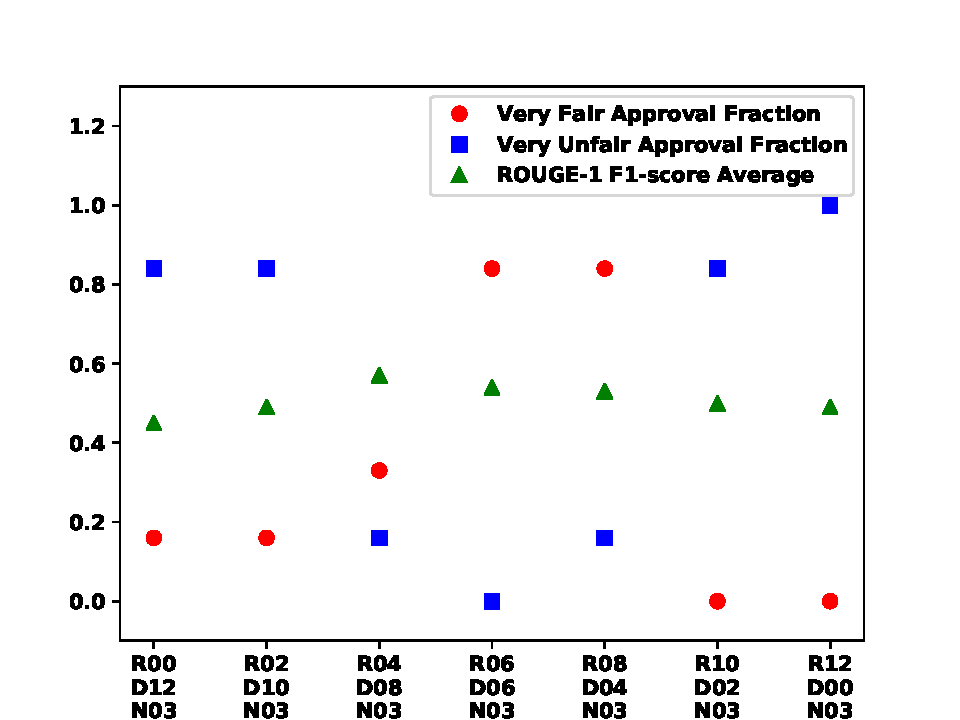
\includegraphics[width=\textwidth, height=3cm]{figures/Sheet2.pdf}
		%\vspace*{-3.5mm}
		\caption{FairSumm-US-Batch1 summaries}
		\label{Fig: RougeApprovalUSEBatch1}
	\end{subfigure}%
	\hfill
	~\begin{subfigure}{0.65\columnwidth}
		\centering
		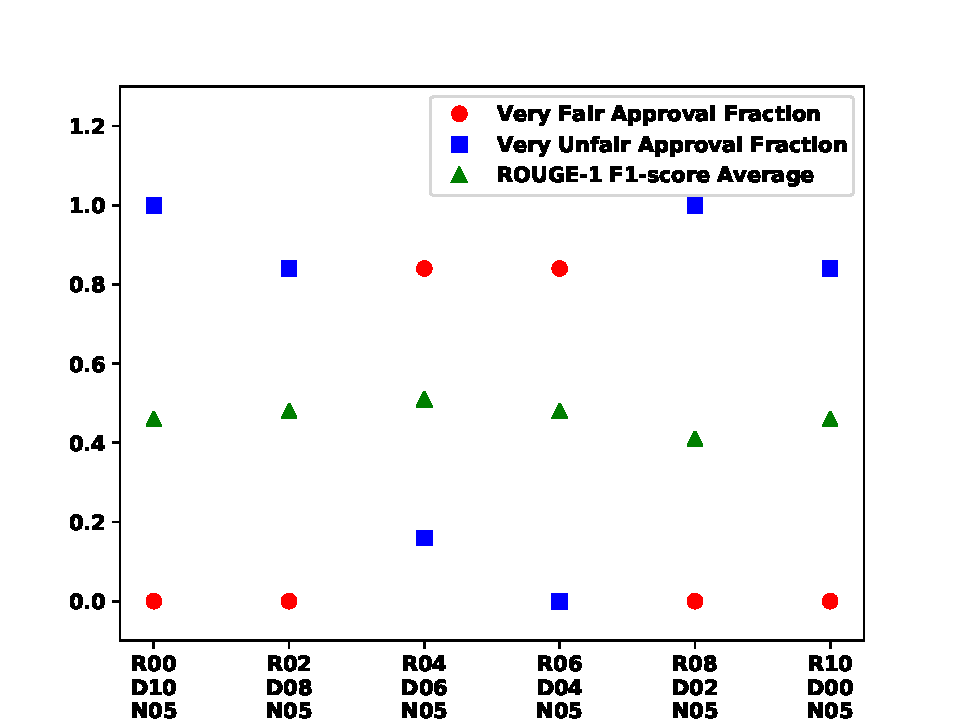
\includegraphics[width=\textwidth, height=3cm]{figures/Sheet6.pdf}
		\vspace*{-3.5mm}
		\caption{FairSumm-US-Batch2 summaries}
		\label{Fig: RougeApprovalUSEBatch2}
	\end{subfigure}
	%\vspace*{-2mm}
	\hfill
	~\begin{subfigure}{0.65\columnwidth}
		\centering
		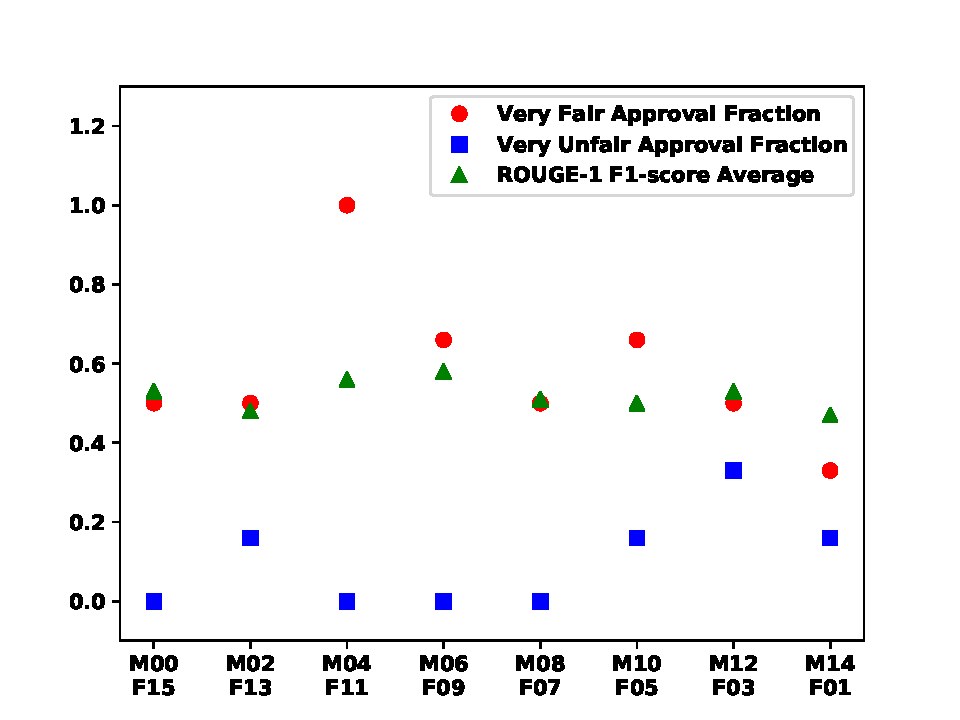
\includegraphics[width=\textwidth, height=3cm]{figures/Sheet10.pdf}
		\vspace*{-3.5mm}
		\caption{FairSumm-MeToo summaries}
		\label{Fig: RougeApprovalMeToo}
	\end{subfigure}
	%\vspace*{-1mm}
	\caption{{\bf ROUGE-1 F1-score values for the different summaries (shown by green triangular markers), along with the very fair/unfair approval fractions for the three batches of summaries. In general ROUGE-1 scores have poor correlation with the fairness approval scores, and hence are not a good indicator of fairness of an algorithmic summary.}} 
	\label{Fig: RougeApproval}
	%\vspace*{-5mm}
\end{figure*}


\vspace{3mm}
\noindent {\bf Computing ROUGE scores:}
We consider the summaries written by the human annotators as `gold standard summaries' and measure the average ROUGE-1 F1 score (based on overlap of unigrams) of all the different summaries in the FairSumm-US-Batch1, FairSumm-US-Batch2 and FairSumm-MeToo batches. 

Note that ROUGE-1 F1 score is computed for an algorithmic summary individually with every gold standard summary (written by a human annotator), and then the average score across all gold standard summaries is considered -- this is in accordance with the standard procedure for evaluation of summaries.
%Specifically, for calculation of ROUGE scores for the USElection dataset, we use $30$ gold standard summaries ($15$ written by  left-leaning AMT workers and $15$ written by right-leaning AMT workers).
%For calculation of ROUGE scores for the MeToo dataset, we used $10$ gold standard summaries ($5$ written by male annotators and $5$ written by female annotators). 


\vspace{3mm}
\noindent {\bf Agreement of ROUGE scores with consumers' perception of fairness in summaries:}
Figure~\ref{Fig: RougeApproval} shows the average ROUGE-1 F1 scores (shown by green triangular markers) obtained by the different summaries in the FairSumm-US-Batch1, FairSumm-US-Batch2 and FairSumm-MeToo batches, along with the fraction of annotators who judged the corresponding summaries to be very fair/unfair (as was described in Section~\ref{sec:consumer-perception}).
Visually, the ROUGE scores appear to have low correlation with the consumers’ perception of fairness of the summaries. 
Very unfair/biased summaries are seen to get similar ROUGE scores as very fair/unbiased summaries. For instance, in Figure~\ref{Fig: RougeApproval}(a), a very biased/unfair summary (containing 12 pro-Republican tweets, 0 pro-Democratic tweets and 3 neutral tweets) obtained a very similar ROUGE score as a very fair summary (containing 6 pro-Republican tweets, 6 pro-Democratic tweets and 3 neutral tweets).

\begin{table*}[tb]
    \centering
    \begin{tabular}{|c|c|c|c|}
    \hline	
     Correlation between   &  FairSumm-US-Batch1 & FairSumm-US-Batch2 & FairSumm-MeToo\\
       \hline \hline
   
    % Rouge-1 F1-core \& Very Unfair Approval Fraction & $-0.82$ & $-0.69$ & $-0.46$ \\
    %\hline
     Rouge-1 F1-score \& Very Fair Approval Fraction & 0.51  & 0.61 & 0.64\\
     \hline
%    \hline
     Perceived Opinion Bias Scores \& Very Unfair Approval Fraction & 0.84 & 0.74 & 0.94\\
     \hline
     Perceived Opinion Bias Scores \& Opinion Interaction Graph scores & 0.96 & 0.94 & 0.93\\
     \hline
    \end{tabular}
    \caption{\bf Pearson's correlation coefficient between different metrics/scores as measured for the three batches of summaries. While the ROUGE1 scores do {\it not} correlate strongly with the fairness approval fractions (fraction of annotators who judged a summary to be fair), the proposed metric (Perceived Opinion Bias Score) has a much stronger correlation with the bias/unfairness of summaries as judged by the annotators.}
    \label{tab:correlation-values}
\end{table*}

To quantify the agreement of ROUGE scores with consumers' perception of fairness in summaries, we compute the {\it Pearson correlation coefficient} between the average ROUGE-1 F1-score of a summary and the `very fair approval fraction' (the fraction of annotators who judged the summary to be very fair).
The Pearson correlation coefficients for the three batches of summaries are shown in Table~\ref{tab:correlation-values} (first row).
We observe the Pearson correlation coefficients to be moderate, in the range $[0.5, 0.65]$, for all three batches.

These results show that the popular ROUGE metrics do {\it not} correlate well with the fairness of summaries as perceived by the consumers.

\section{Metric for Capturing Consumers' Perception of Opinion Bias}
\label{sec:bias-metric}


\noindent
Having established that the popular ROUGE scores cannot capture the bias/unfairness in summaries, we now formulate a metric that can capture the bias of summaries with respect to representation of various opinions in the input, as perceived by human annotators. 
In other words, in this section, we study \textbf{RQ$3$} as mentioned in the introduction.%Section \ref{sec: intro}. 

In brief, our proposed bias metric is based on first asking human annotators to identify the set of distinct opinions in the given input text (which is to be summarized), and then checking how well the different opinions are represented in a particular summary. We describe the setup below in detail.

We go back to the survey described in Section~\ref{sec:consumer-perception} where a set of $N=6$ annotators (say, $A_1, A_2, \ldots, A_N$) were asked to identify all the distinct opinions being conveyed by an input set of tweets.
We consider the union of all distinct opinions identified by all the annotators. 
Let the set of all distinct opinions (in the input text) be denoted by $O$, and assume that there are $k$ distinct opinions $O_1, O_2, ..., O_k$.

% Let us call this set $O$ with cardinality of this set being $k$ if it contains $k$ units of opinions within it $O_1$, $O_2$,.., $O_k$. Let the set of annotators be called annotator set A, with its cardinality being 6; $A_1$, $A_2$,..,$A_6$.   


In an extension of that survey, the annotators were shown the set $O$ of all distinct opinions, and all the summaries (from the batches FairSumm-US-Batch1, FairSumm-US-Batch2 and FairSumm-MeToo) in random order.
For each summary, all the $N=6$ annotators were asked to label whether the summary adequately represents each of the distinct opinions.
More formally, with respect to a particular summary $S$ (that is to be evaluated), we ask each annotator $A_i$ to label each opinion $O_j$ as one of the following, based on which the function $G_{ij}$ is defined as follows -- 
\begin{enumerate}
    \item The opinion $O_j$ is completely represented in the summary $S$ $ \implies G_{ij}(S) = 1.0$
    \item The opinion $O_j$ is somewhat adequately represented in the summary $S$ $ \implies G_{ij}(S) = 0.5$
    \item The opinion $O_j$ is inadequately represented in the summary $S$ $ \implies G_{ij}(S) = -0.5$
    \item The opinion $O_j$ is completely absent in the summary $S$ $ \implies G_{ij}(S) = -1.0$
\end{enumerate}

\if 0 

Let us define an arbitrary function $f$ for converting the annotation given by participants to numerical values

$f$(relatively fair)= $1.0$

$f$(somewhat fair)= $0.5$

$f$(relatively unfair)= $-0.5$

$f$(totally unfair representation)= $-1.0$

For a given summary, let $G_{ij}$ represent annotation given by annotator $A_i$ for opinion $O_j$. 

\fi



\begin{figure*}[h]
	\centering
	\begin{subfigure}{0.65\columnwidth}
		\centering
		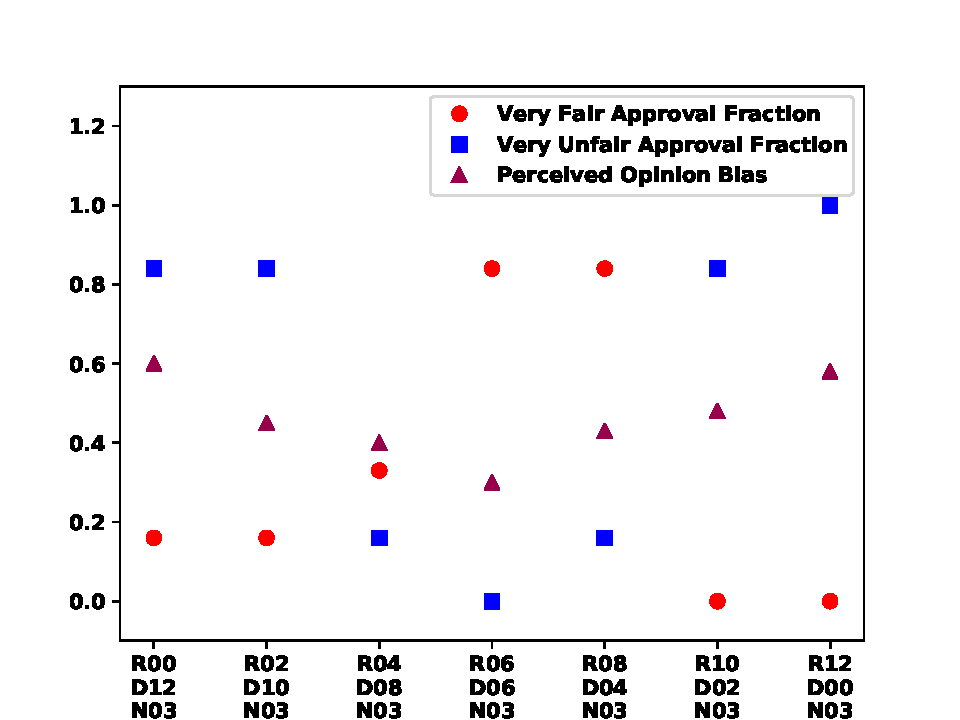
\includegraphics[width=\textwidth, height=3cm]{figures/Sheet3.pdf}
		%\vspace*{-3.5mm}
		\caption{FairSumm-US-Batch1 summaries}
		\label{Fig: HumanApprovalUSEBatch1}
	\end{subfigure}%
	\hfill
	~\begin{subfigure}{0.65\columnwidth}
		\centering
		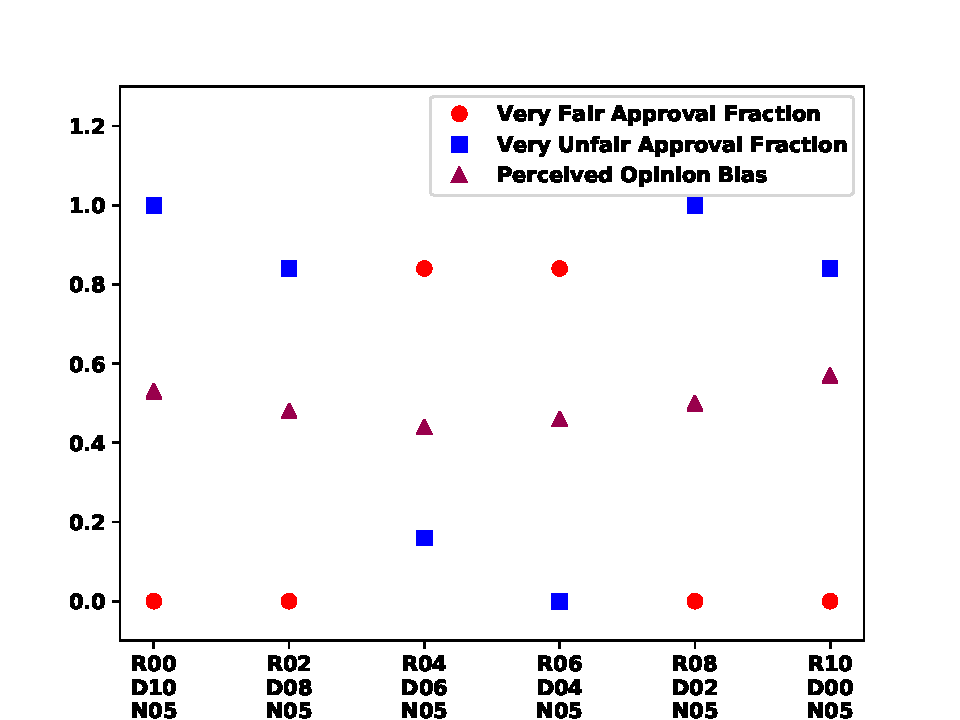
\includegraphics[width=\textwidth, height=3cm]{figures/Sheet7.pdf}
		\caption{FairSumm-US-Batch2 summaries}
		\label{Fig: HumanApprovalUSEBatch2}
	\end{subfigure}
	%\vspace*{-2mm}
	\hfill
	~\begin{subfigure}{0.65\columnwidth}
		\centering
		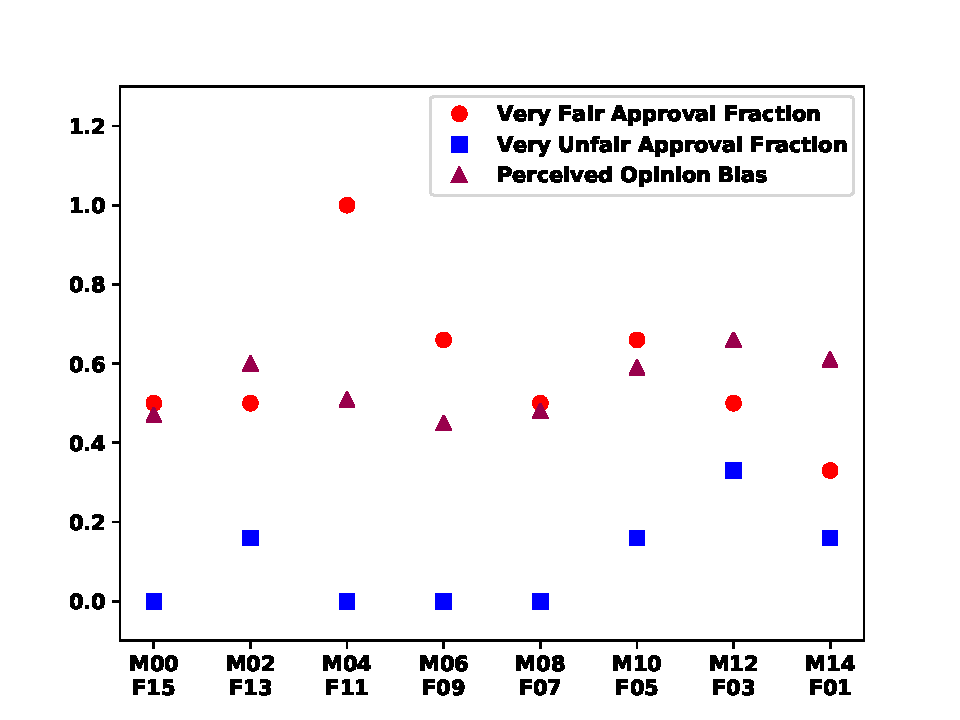
\includegraphics[width=\textwidth, height=3cm]{figures/Sheet11.pdf}
		\caption{FairSumm-MeToo summaries}
		\label{Fig:HumanApprovalMeToo}
	\end{subfigure}
	%\vspace*{-1mm}
	\caption{{\bf Perceived Opinion Bias scores (shown by the triangle markers) along with the approval fractions for the three batches of summaries. The Perceived Opinion Bias scores have good agreement with the `very unfair approval fractions'. In other words, the summaries that are judged to be unfair by a high (respectively, low) fraction of annotators have high (respectively, low) Perceived Opinion Bias scores.}} 
	\label{Fig:perceived-opinion-bias}
	\vspace*{-3mm}
\end{figure*}


We define the {\it cumulative representation score} $C_j$  obtained by the opinion $O_j$ in summary $S$ as the mean of all the $G_{ij}$ scores given by all the annotators:
\begin{equation}
   C_j(S) = \frac{1}{N} \sum_{i=1}^N G_{ij}(S)
\end{equation}
Intuitively, $C_j(S)$ denotes how well the opinion $O_j$ is represented in the summary $S$, as judged by all the annotators.

Finally we define the {\it Perceived Opinion Bias} of summary $S$ as the Gini coefficient of the cumulative representation score of all the distinct opinions.
So for a given summary $S$, the perceived opinion bias of $S$ is computed as Gini Coefficient($C_1(S)$, $C_2(S)$,..,$C_k(S)$).
The motivation for using the Gini coefficient is as follows.
The Gini coefficient has been originally used to measure the income inequality or wealth inequality within a group of people (e.g., the people in a certain country). 
Here we apply the Gini coefficient to measure the inequality of representation/exposure within the set of distinct opinions.
If different opinions get widely different amounts of representation/exposure in a summary $S$, then $S$ is biased towards some of the opinions, and hence the Perceived Opinion Bias score of $S$ will be high.


\vspace{3mm}
\noindent {\bf Agreement of Perceived Opinion Bias scores with consumers' perception of unfairness:}
Now we investigate whether our proposed Perceived Opinion Bias scores agree with the consumers' perception of bias/unfairness of summaries. 
Figure~\ref{Fig:perceived-opinion-bias} depicts the perceived opinion bias scores and the very fair/unfair approval fractions (see Section~\ref{sec:consumer-perception} for the definition of these fractions) for the three batches of summaries. 
From the plots, it is evident that there is a good agreement between the perceived opinion bias and the `very unfair approval fraction'.
In other words, those summaries that are judged to be {\it very unfair} by a large fraction of annotators get high Perceived Opinion Bias scores.
In contrast, those summaries that are judged to be {\it very fair} by a large fraction of annotators get low Perceived Opinion Bias scores.




To quantify the agreement, we also compute the Pearson correlation coefficient between the Perceived Opinion Bias score of a summary and the `very unfair approval fraction' (the fraction of annotators who judged the summary to be very unfair).
The Pearson correlation coefficients for the three batches of summaries are shown in Table~\ref{tab:correlation-values} (second row).
For every batch of summaries, we observe the Pearson correlation coefficients to be substantially higher than the corresponding correlation coefficients for the ROUGE F1-scores.\footnote{Note that ROUGE scores are supposed to be higher for good summaries; hence we measure correlation with `very fair approval fraction. In contrast, the Perceived Opinion Bias scores are supposed to be higher for biased/unfair summaries; hence we measure correlation with `very unfair approval fraction'.}
These results show that the proposed Perceived Opinion Bias scores can be used as more reliable measures of bias/unfairness in summaries, than the ROUGE scores.

While the utility of the Perceived Opinion Bias scores is clear, a lot of human annotation effort is needed in computing these scores (first identifying the distinct opinions, and then judging the representation of each opinion in the summary).
Hence the approach of directly computing Perceived Opinion Bias scores may not be scalable to really large datasets.
In the next section, we attempt to develop an {\it automated} methodology for computing the bias/unfairness of summaries.



\section{An Automated Approach to Quantify \\ Consumers' Perceived Bias in Summaries}
%Human evaluation, if done properly, is the ideal way for measuring bias/fairness. However, this approach requires lot of manual effort, and hence does not scale well.
\noindent
In this section, we present an automated method to compute the bias/unfairness of summaries.
Our proposed method, inspired by~\cite{concept-interaction-graph}, represents the input text (a document $d$) as an undirected and weighted network/graph, called the {\it Opinion Interaction Graph} ($OIG$). 
%A $OIG$ is a graph $G_d$, where each vertex/node is an opinion which is a keyword or a set of highly correlated keywords appearing in the input text. 
%The input text is first decomposed into subsets of sentences, each subset focusing on a different opinion. 
%The opinion expressed in a sentence will be used for attaching it to a particular opinion-vertex that it is most related to. 
%Hence, opinion-vertices will have their own sentence sets, which are disjoint. 
%The opinion-vertices are connected with weighted edges.
%The weight of the edge between a pair of opinion-vertices denotes how much the two opinions are related to each other and can be determined in various ways. 
We now describe the various steps of the algorithm in detail.

\subsection{The algorithm}

\vspace{2mm} \noindent 
\textbf{Step 1: Generation of Key graph:}
Given the input text, we first extract the named entities and keywords by the TextRank algorithm.
Then we construct a {\it keyword co-occurrence graph}, called {\bf KeyGraph}, based on the set of extracted keywords. Each keyword is a vertex in the KeyGraph. 
We connect two keywords by an edge if they co-occur in the same sentence. The edge between two keywords is weighted by frequency of co-occurrences of the two said keywords.



\begin{figure*}[t]
	\centering
	\begin{subfigure}{0.65\columnwidth}
		\centering
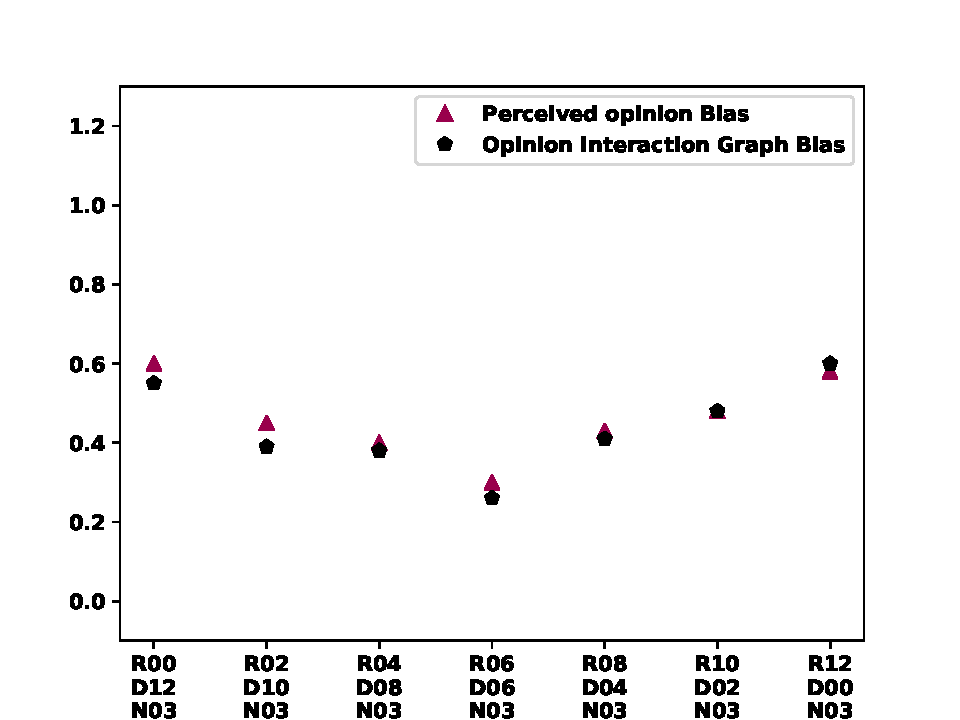
\includegraphics[width=\textwidth, height=3cm]{figures/Sheet4.pdf}
		%\vspace*{-3.5mm}
		\caption{FairSumm-US-Batch1 summaries}
		\label{Fig: GraphBiasScoreUSEBatch1}
	\end{subfigure}%
	\hfill
	~\begin{subfigure}{0.65\columnwidth}
		\centering
		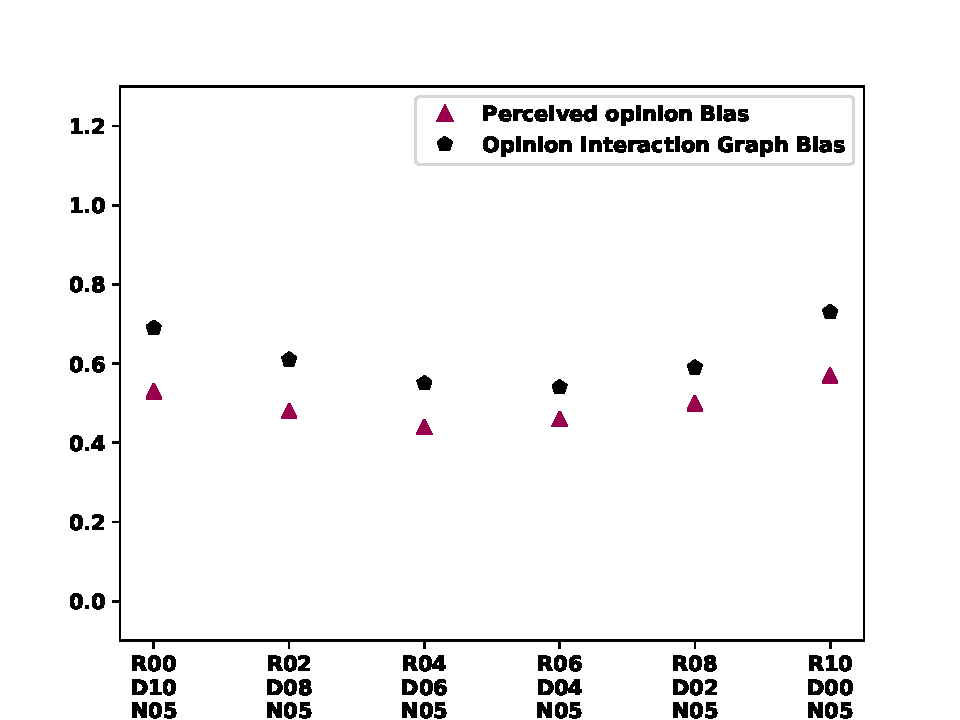
\includegraphics[width=\textwidth, height=3cm]{figures/Sheet8.pdf}
		%\vspace*{-3.5mm}
		\caption{FairSumm-US-Batch2 summaries}
		\label{Fig: GraphBiasScoreUSEBatch2}
	\end{subfigure}
	%\vspace*{-2mm}
	\hfill
	~\begin{subfigure}{0.65\columnwidth}
		\centering
		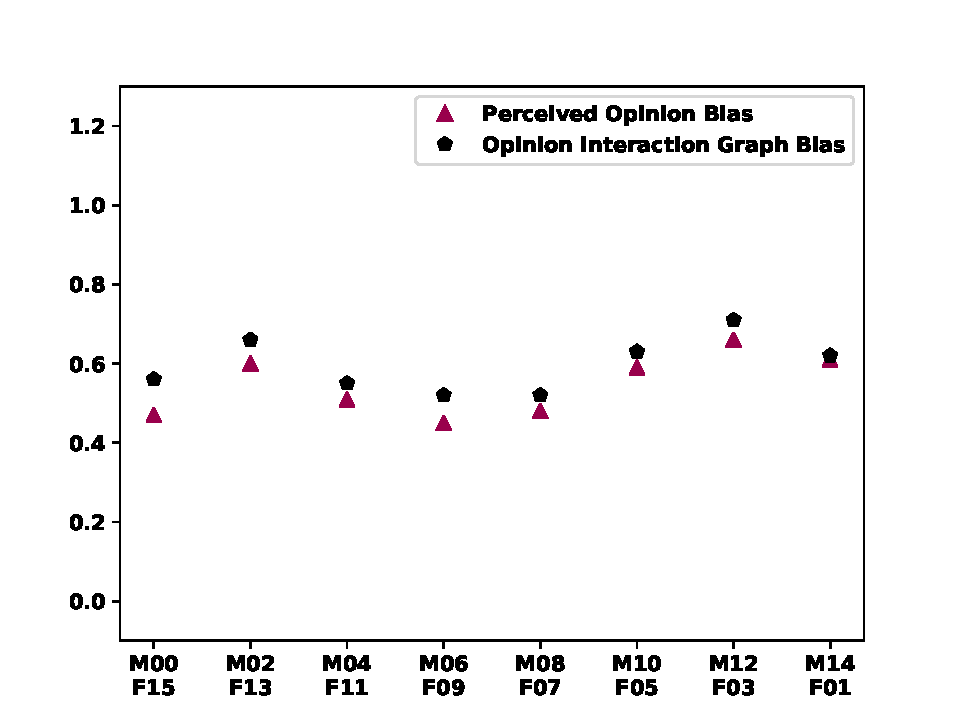
\includegraphics[width=\textwidth, height=3cm]{figures/Sheet12.pdf}
		%\vspace*{-3.5mm}
		\caption{FairSumm-MeToo summaries}
		\label{Fig: GraphBiasScoreMeToo}
	\end{subfigure}
	
	\caption{{\bf Opinion Interaction Graph scores (computed automatically) along with Perceived Opinion Bias scores (computed based on human annotation) for the three batches of summaries. The two scores have very high agreement, thus establishing that our methodology based on Opinion Interaction Graph can be used to automatically measure the Perceived Opinion Bias of summaries.}} 
	\label{Fig: GraphBiasScore}
	%\vspace*{-5mm}
\end{figure*}

\vspace{2mm} \noindent 
\textbf{Step 2: Concept Detection:}
The structure of KeyGraph reveals the connections between keywords. If a subset of keywords are highly correlated, they will form a densely connected subgraph in  KeyGraph, which we call an {\it opinion}.\footnote{Intuitively, the idea is similar to what is followed in topic modeling, where each topic is essentially a set of frequently co-occurring terms.} 
Opinions can be extracted by applying {\it community detection algorithms} on the KeyGraph. 
A Community Detection algorithm is used to split a KeyGraph  into a set of communities $O$ = \{$O_1$, $O_2$, .., $O_{|O|}$\}, where each community $O_i$ contains the keywords related to a certain opinion. 
%For this purpose we obtain an adjacency matrix for the nodes of the key graph and the row vector of the matrix becomes a vector representation of the corresponding key. 
To this end, we use the popular Louvain community detection algorithm~\cite{blondel-louvain} for clustering the KeyGraph into fixed sized  communities. However, other clustering methods can also be used in this step. 

\vspace{2mm} \noindent 
\textbf{Step 3: Sentence Attachment and Edge Construction:}
After the opinions are discovered, the next step is to associate sentences to opinions. We calculate the cosine similarity between each sentence and each opinion, where sentences and opinions are represented by TF-IDF vectors of the words. 
We assign each sentence to that opinion $O_i$ which is the most similar to the said sentence, where the similarity is computed based on what fraction of the keywords associated with an opinion is contained in the said sentence.
%Emayqual Representation. This rides on the premise that all opinions have an equal right to be exposed in the final summary. The exposure that an opinion gets is therefore proportional to the relative  abundance of sentences related to that opinion vis-a-vis other opinions in the summary. 
The sentences that do not match any opinion in the document will be attached to a dummy vertex that does not contain any keywords. 

Then we construct the Opinion Interaction Graph $OIG$ where each vertex/node is an opinion.
To construct edges that reveal the similarity between different opinions, for each vertex, we represent its associated set of sentences as a concatenation of the sentences attached to it. The edge weight between two vertices is computed as the TF-IDF similarity between their associated sentence sets.

\vspace{2mm} \noindent 
\textbf{Step 4: Computing exposure of an opinion in a summary:}
As of now, we have constructed the $OIG$ where every node is an opinion and is associated with a set of sentences. Next we quantify the representation/exposure of different opinions in a given summary $S$ (which is to be evaluated).
We simply compute the exposure of an opinion as the fraction of the sentences attached to the said opinion, that is present in the summary $S$.\footnote{Note that more complex models can be applied to compute the exposure of opinions, e.g., a part of the exposure of $O_j$ can be thought to diffuse to another very similar opinion $O_j$, where the similarity between the two opinions is quantified by the edge-weight in the $OIG$.
%Further, the exposure may also be updated through diffusion. 
However, we have avoided such complexities in order to keep our model simple.}


%We start with a hypothesis that if sentence/sentences from a concept is/are present in a summary S they get some exposure. To quantify the exposure, we may rely on two subtypes of ‘group fairness’ as explained in section 2.2. Equal Representation: This rides on the premise that all opinions have an equal right to be exposed in the final summary. The exposure that an opinion gets is therefore proportional to the relative  abundance of sentences related to that opinion vis-a-vis other opinions in the summary. 

%Proportional Representation: The foundational argument here is that the distribution of exposure should mimic the distribution of sentences attached to opinions in the original document. We deal with proportional representation in this work. So,


\vspace{2mm} \noindent 
\textbf{Step 5: Quantifying the skew in the distribution of exposure:} 
Finally, we compute the Gini coefficient of the exposure received by all the distinct opinions (as computed above) to quantify the bias in the distribution of exposure of different opinions in the summary $S$.
The intuition behind using the Gini coefficient has been discussed in Section~\ref{sec:bias-metric}.

It can be noted that, intuitively, we adhere to the {\it proportional representation notion of fairness} (that was explained in Section~\ref{sub:fairness-notions}) among the exposures obtained by different opinions. 
In other words, a summary would be considered most fair if the distribution of exposure received by the various opinions resembles the distribution of sentences attached to the opinions.





\subsection{Results based on opinion interaction graph}
\noindent
Figure~\ref{Fig: GraphBiasScore}
shows the bias of the various summaries in the three batches, as computed by our proposed Opinion Interaction Graph algorithm, and the Perceived Opinion Bias scores of the summaries as obtained in the previous section. 
It is evident that there is a very high correlation between the metrics.

Also Table~\ref{tab:correlation-values} (last row) shows the Pearson correlation for the Perceived Opinion Bias scores and the bias scores computed by the OIG-based method. For all three batches of summaries, the correlation scores are above $0.9$.

These results show that our proposed graph-based algorithm is a good proxy for automatic calculation of perceived opinion bias of summaries.


\section{Conclusion}
\noindent
To our knowledge, this work is the first attempt to explore fairness in the context of automatic summarization from the perspective of consumers/readers of the summary. 
We show that the notion of fairness in summaries from the consumers' perspective varies from one context to another (e.g., may correspond to fair representation of demographic groups of the producers/writers, or the fair representation of opinions from the input text).
Also the popular ROUGE metrics for evaluation of summaries usually cannot capture the fairness of summaries.
To bridge this gap, we have proposed an alternative metric for measuring the bias in summaries (based on human annotation), as well as an automatic  methodology to approximate the metric.

We believe that this work has several potential applications in areas where the text to be summarized consists of multiple different perspectives or opinions, e.g., in news article summarization, debate summarization, and so on.
We plan to explore such applications in future. 
Also, we plan to develop metrics that can simultaneously capture both the quality and the fairness of summaries, e.g., by suitably combining the ROUGE metrics with the bias metric proposed in this work.




\if 0

% use section* for acknowledgment
\ifCLASSOPTIONcompsoc
  % The Computer Society usually uses the plural form
  \section*{Acknowledgments}
\else
  % regular IEEE prefers the singular form
  \section*{Acknowledgment}
\fi

\fi

\section*{Acknowledgments}
\noindent
The authors would like to thank the annotators who judged the summaries as part of the work. 
This research was supported in part by a European Research Council (ERC) Advanced Grant for the project ``Foundations for Fair Social Computing'', funded under the EU Horizon 2020 Framework Programme (grant agreement no. 789373). 
A. Dash was supported by a fellowship from Tata Consultancy Services.





% trigger a \newpage just before the given reference
% number - used to balance the columns on the last page
% adjust value as needed - may need to be readjusted if
% the document is modified later
%\IEEEtriggeratref{8}
% The "triggered" command can be changed if desired:
%\IEEEtriggercmd{\enlargethispage{-5in}}

% references section

% can use a bibliography generated by BibTeX as a .bbl file
% BibTeX documentation can be easily obtained at:
% http://mirror.ctan.org/biblio/bibtex/contrib/doc/
% The IEEEtran BibTeX style support page is at:
% http://www.michaelshell.org/tex/ieeetran/bibtex/
%\bibliographystyle{IEEEtran}
% argument is your BibTeX string definitions and bibliography database(s)
%\bibliography{IEEEabrv,../bib/paper}
%
% <OR> manually copy in the resultant .bbl file
% set second argument of \begin to the number of references
% (used to reserve space for the reference number labels box)

\bibliographystyle{IEEEtran}
\bibliography{fairness.bib}

\end{document}